\documentclass[12pt]{article}
\usepackage[utf8x]{inputenc}
\usepackage{hyperref}
\usepackage{amsmath}
\usepackage{graphicx}
\usepackage[colorinlistoftodos]{todonotes}
\usepackage[toc,page]{appendix}
\usepackage{smartdiagram}
\usepackage{indentfirst}


\usetikzlibrary{fit}


\begin{document}
\graphicspath{{images/}}
\begin{titlepage}

\newcommand{\HRule}{\rule{\linewidth}{0.5mm}} % Defines a new command for the horizontal lines, change thickness here
\setlength{\topmargin}{0in}
\center % Center everything on the page


 \begin{minipage}{0.4\textwidth}
\begin{flushleft} \large
\hspace*{-0.5cm}

\includegraphics[scale=0.4]{images/imag.jpg}\\
\end{flushleft}
\end{minipage}
~
\begin{minipage}{0.5\textwidth}
\begin{flushright} \large
\hspace*{2cm}

\includegraphics[scale=0.4]{images/company.png}\\
\end{flushright}
\end{minipage}\\[1cm]
%----------------------------------------------------------------------------------------
%	HEADING SECTIONS
%----------------------------------------------------------------------------------------

\textsc{\LARGE Université Grenoble Alpes}\\[1.5cm]
\textsc{\Large Master 2 Génie Informatique}\\[0.5cm]
\textsc{\large Mémoire d'Alternance}\\[0.5cm]

%----------------------------------------------------------------------------------------
%	TITLE SECTION
%----------------------------------------------------------------------------------------

\HRule \\[0.4cm]
{ \huge \bfseries Ingénieur DevOps}\\[0.4cm]
\HRule \\[1cm]

%----------------------------------------------------------------------------------------
%	AUTHOR SECTION
%----------------------------------------------------------------------------------------

\begin{minipage}{0.4\textwidth}
\begin{flushleft} \large
\emph{Author:}\\
Gerardo \textsc{LARREINEGABE} \\
\end{flushleft}
\end{minipage}
~
\begin{minipage}{0.5\textwidth}
\begin{flushright} \large
\emph{Maître d’apprentissage:} \\
Duy \textsc{Tran Quang} \\[0.5cm] % Supervisor's Name
\emph{Tuteur Pédagogique:} \\
Olivier \textsc{Gruber} % Supervisor's Name
\end{flushright}
\end{minipage}\\[1cm]

%----------------------------------------------------------------------------------------
%	DATE SECTION
%----------------------------------------------------------------------------------------

{\large Grenoble, le 25 août 2018}\\[0.5cm]


\vfill % Fill the rest of the page with whitespace

\end{titlepage}

\renewcommand{\abstractname}{Résumé}
\begin{abstract}
\noindent
Dans le cadre de mon alternance, j'ai intégré l'équipe de IT au sein de
la société Bonitasoft, qui gère plusieurs projets dont BCD forme part et vise
à fournir au client une solution DevOps et des bonnes pratiques pour aboutir
à la Livraison Continue des applications créés avec Bonita.
Le nom BCD est l'acronyme en anglais de \textbf{Bonita Continuous Delivery}. \\
BCD aborde actuellement deux problèmes communs des développeurs qui est la \emph{création}
d'un environnement normalisé et le \emph{déploiement} d'une application Bonita.\\ \\
\textbf{\textit{Mot clés:} livraison continue, déploiement, devops, bonita
création d’environnement}
\end{abstract}

\newpage
\setcounter{tocdepth}{2}
\tableofcontents
\newpage

\section{Introduction}
Dans le cadre de mon alternance, j'ai occupé un poste d'Ingénieur DevOps dans l'entreprise Bonitasoft.
Pour commencer, je présenterai mon entreprise, l'organisation, les différentes équipes de travail, la méthode de travail de façon générale.
En deuxième partie, je mettrai un accent sur l'équipe avec laquelle j'ai collaboré, l'organisation interne, la façon de travailler et les activités que l'équipe mène tous les jours.
En troisième, j'exposerai le projet sur lequel j'ai travaillé, la problématique, et les objectifs de mon sujet, ainsi que les différentes techniques requises pour les accomplir.

\section{Environnement Professionnel}
\subsection{L'entreprise}
\subsubsection{Mission-Vision}
De la démocratisation du BPM à la transformation numérique en profondeur de l'entreprise, nous sommes à la pointe d'une révolution professionnelle depuis que notre entreprise a vu le jour.
Le succès de nos clients est notre succès, et tout le monde chez Bonitasoft est un contributeur, chaque jour.
\cite{Bonitasoft2017BONITA1}

\subsection{Un peu d'Histoire}
Bonitasoft est un éditeur de logiciel open source créé en 2001. Il a commencé comme
Bonita BPM dans l'Institut National de Recherche en Informatique et en
Automatique (INRIA) puis transféré au Groupe Bull.
En 2009, Miguel Valdés Faura rejoint Charles Souillard et Rodrigue Le Gall pour
fonder Bonitasoft.
En 2011, après une série de levée de fonds, Bonitasoft a pu commercialiser son
produit Bonita à l'international et le premier bureau de Bonitasoft est ouvert
aux Etats-Unis.\cite{wikipedia_2018}



\subsection{Organisation}
Bonitasoft a quatre bureaux principaux, aux États-Unis, à San Francisco et à New York,
en France à Paris et à Grenoble.
Les activités sont organisée et divisée en 5 different services:


\begin{center}
  \smartdiagramset{bubble node size=4cm, bubble center node size=6cm}
  \smartdiagram[bubble diagram]{Bonitasoft,
  IT,Service Professionnel,
  R\&D, Support, Succès du Client}
\end{center}


\subsubsection{IT}
Le département de l'IT est le gardian principal de tout le tâches IT commun comme:
\begin{itemize}
  \item La gestion des environnements virtuels. (cloud ou serveur physique).
  \item La gestion de l'automatisation de processus de CI interne.
  \item La gestion des licences des applications payent (OS, applications).
  \item La gestion des appareils, périphériques, les ordinateurs portables,
  \item L'architectures, méthodologies et règles régissant l'utilisation et le stockage des données.
  \item L'administration de systèmes: la configuration, gestion, entretien et dépanne des environnement
  informatique multi-utilisateur (cloud ou physique).
  \item  La gestion ou l'aide aux autres département avec la culture et pratiques DevOps.
\end{itemize}

Aussi, l'équipe d'IT de Bonitasoft gère d'autres projets comme:
\begin{itemize}
  \item Salesforce: depuis la création des use cases jusqu'à la mise en production en garantissant la gouvernance du système avec une approche DevOps.
  \item BCD: c'est une solution fournit pour utiliser les bonnes pratiques DevOps pour la livraison continue (CI) d'une application Bonita.
\end{itemize}

L'équipe est composée de quatre personnes, dont l'une est moi.

\begin{figure}[h]
  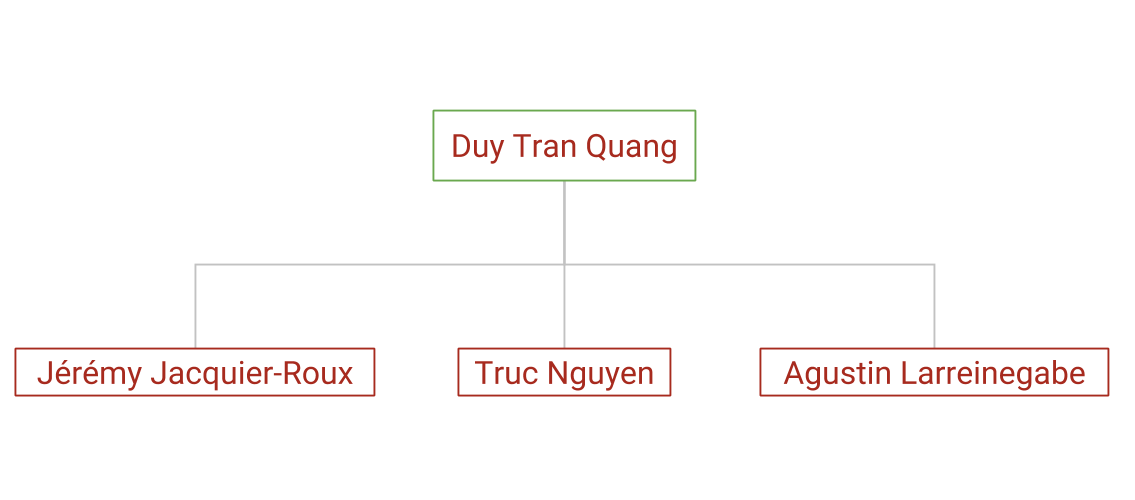
\includegraphics[width=\textwidth,keepaspectratio]{it_team.png}
   \caption{Organigramme.}
   \label{figure:organigrame}
\end{figure}

\subsubsection{R\&D}
Il est le plus grand département et son travail principal est le développement de la plate-forme Bonitasoft.
Il est divisé par équipes de travail ou projets:
\begin{itemize}
  \item Back-end
  \item Front-end
  \item BICI, c'est une application autonome connectée au moteur de Bonita qui permet d'analyser l'exécution
   des processus et prévoir et améliorer l'efficacité de l'équipe.
\end{itemize}

\subsubsection{Customer Success (CS)}
Le département gère la relation entre Bonitasoft et ses clients. L'objectif de la réussite du client est de rendre le client le plus performant possible, ce qui, à son tour, améliore la valeur à vie du client pour l'entreprise.
Cette fonction est la plus couramment utilisée dans le monde du logiciel et la plus répandue parmi les sociétés de services. Parce que le succès du client est un domaine naissant, son alignement organisationnel et ses activités sont toujours en évolution.

\subsubsection{Support}
Ce département est en charge de traiter et de diriger les différentes questions et problématiques du client.
Chaque problème ou bogue est chargé dans l'outil Jira et traité par le département R\&D ou l'IT.
Chaque ticket chargé a une priorité et il est résolu par ordre de priorité.

\subsubsection{Service Professionnel}
C'est une équipe d'experts qui offre de la valeur pour le succès du client en suivant les projets depuis le début avec la meilleure expérience-utilisateur possible.



\section{Produits} \label{produits}
Actuellment, l'entreprise a une produit principal qui est \emph{Bonita}, et deux produits complémentaire qui sont \textit{Bonita Continuous Delivery} et \textit{Bonita Intelligent Continuous Improvement}

Dans cette partie, nous allons introduire de manière superficiel tous les produits pour avoir un contexte plus claire de la mission.

\begin{figure}[!ht]
\centering
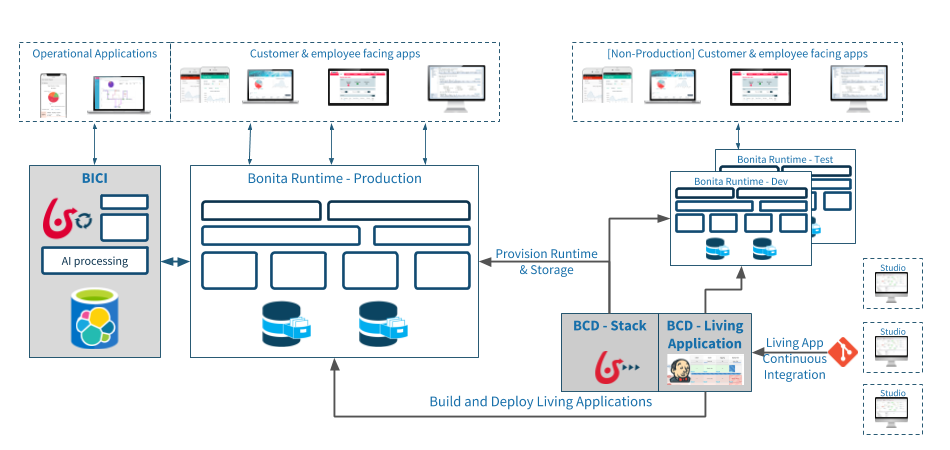
\includegraphics[scale=0.39]{bonita_add-on_archi.png}
\caption{Interaction entre Produits}
\label{fig:bonita_add-on}
\end{figure}

\subsection{Bonita}
\begin{quotation}
Le BPM est la discipline de la gestion des processus (plutôt que des tâches) en tant que moyen d'améliorer les résultats de performance de l'entreprise et l'agilité opérationnelle. \cite{gartnerdic}
\end{quotation}

Bonita est une plate-forme basé sur BPM qui sert à construire des applications, personnalisées, en prenant l'avantage plein du BPM pour s'adapter aux changements en temps réel.

La plate-forme a deux parties. Voir Figure \ref{fig:bonita_archi}:
\begin{itemize}
  \item Bonita Studio
  \item Bonita Plate-forme (Bonita Engine)
\end{itemize}

\subsubsection{Bonita Studio}
Bonita le Studio est un environnement graphique pour créer des processus, des applications, des modèles de données et des vues d'utilisateurs. Il contient trois outils de design(conception) majeurs:

\begin{itemize}
  \item Le tableau blanc, pour dessiner un organigramme de processus et définir les transitions.
  \item Le menu de Développement, pour étendre les capacités du Studio et crée les modèles de données.
  \item Le Concepteur UI, qui est utilisé pour créer des pages d'application et des formulaires de processus
\end{itemize}

Le Studio contient une Plate-forme Bonita (Tomcat, UI Designer, Bonita Portal, Bonita Engine et une base de données H2), approprié pour tester une application

\subsubsection{Bonita Engine}
C'est le runtime processeur au cœur de Bonita. Il exécute des processus, en traitant des actions liées aux tâches, comme l'accès de base de données. Le Moteur est composé d'un certain nombre de services et API. Les services sont services BPM ou des services génériques.

\begin{figure}[!ht]
\centering
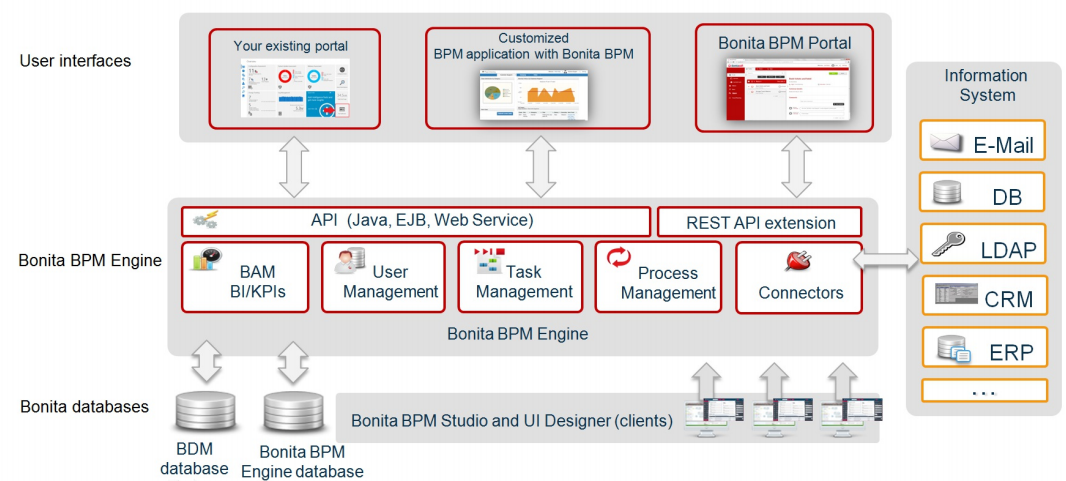
\includegraphics[scale=0.5]{bonita_archi.png}
\caption{Bonita Architecture}
\label{fig:bonita_archi}
\end{figure}

\subsection{Bonita Continuous Delivery (BCD)} \label{bcd}
Bonita Continuos Delivery ou \textit{BCD} est une solution qui permet l'intégration continue d'une application Bonita en promouvant aussi des bonnes pratiques \emph{DevOps}

Au début, BCD a démarré à partir d'un besoin interne de tester plus facilement des développements. La mise en place d'un environnement avec l'installation de \textit{Bonita Engine} était un processus lent et répétitif, aussi, suite à divers retours des clients, la Directive a décidé de voir comme un potentiel produit.

Actuellement, \textit{BCD} a deux parties. Voir Figure \ref{fig:bcd_cap}:
\begin{itemize}
  \item Livingapp, qui permet la compilation d'un projet avec la gestion de bibliothèques essentielles pour une application \textit{Bonita Subscription}, sans avoir besoin de Bonita Studio, et aussi de déployer l'application compilé dans un stack Bonita configuré.
  \item Stack, qui permet d'un part la création des environnements virtuels dans le cloud (AWS actuellement), et l’installation d'un Stack Bonita dans les serveurs configurés.
\end{itemize}

\begin{figure}[!ht]
\centering
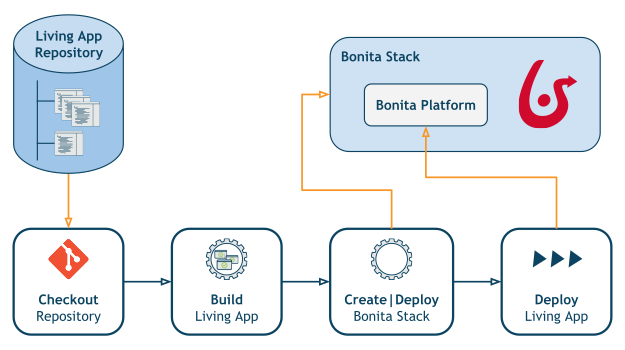
\includegraphics[width=\textwidth,keepaspectratio]{bcd_capabilities.png}
\caption{Fonctionnalités BCD}
\label{fig:bcd_cap}
\end{figure}

\subsection{Intelligent Continuous Improvement (ICI)}

ESCRIBIR


\section{Mission}
Le sujet de la mission d’alternance était d'approfondir la culture \emph{DevOps} en mettant en relation avec Ansible, Docker, Jenkins et le cloud avec Amazon AWS sur un rythme Agile \textit{Scrumban} en ayant Python comme langage de base.

Comme nous l’avons déjà vu dans la Section \ref{bcd}, le complément BCD est celui qui aide à implémenter les bonnes pratiques DevOps au client grâce à l'automatisation de la création d'environnements et l'approvisionnement de stack Bonita, et aussi la compilation et le déploiement d'une application Bonita.

Pour continuer, nous allons voir les concepts \emph{DevOps} ciblés par l'applicatif pour donner un cadre théorique, puis on verra plus en détail le travail réalisé cette année d'alternance.

\subsection{Devops}\label{sec:devops}
De nos jours, dans le domaine du numérique, nous livrons une large gamme de services grâce à des expériences numériques, et pour les améliorer, nous devons avoir le retour du client pour pouvoir proposer de nouveaux types d’expériences et de valeurs. Ce faisant, nous allons être plus compétitifs et nous aurons des nouveaux moyen d'interagir avec les clients.

Tout cela, nous pouvons le faire grâce à des bonnes pratiques pour rendre le travail beaucoup plus efficace, pour cela nous allons entrer dans le monde DevOps.

DevOps est avant tout une culture, des pratiques collaboratives et de l'automatisation qui alignent les équipes de développement et d'opération afin qu'elles puissent améliorer leur expérience client, répondre plus rapidement aux besoins et assurer l'innovation \cite{IsaacSacolick2016DrivingCulture}.

Cependant, cela n'est pas seulement une culture, DevOps involucre principalement un changement de base de comment nous gérons nos applications et comment nous les déployions, en investissant dans l'automation et en changeant les application héritées \cite{benjamin_wootton}.

Pour cette raison, quand nous parlons de DevOps, nous avons:

\begin{itemize}
\item L'automatisation de test.
\item Assurer des déploiements plus fréquents et plus fiables.
\item Avoir la clarté de rôles et des responsabilités.
\item Définir l'indicateur de performance \(KPI\) et sa portée.
\item Automatisation et surveillance.
\end{itemize}

Pour commencer, nous devons nous assurer que tous sont alignés sur ce que DevOps signifie et avec un défi et non à l’ensemble des pratiques DevOps.

Nous devons également rester concentrés sur l’assurance qualité (QA) en sachant qu’il s’agit d’une discipline et d’un ensemble de compétences distincts.

Par exemple, dans la Figure \ref{devops_operational_model} nous voyons une modèle opérationnel proposé ou dans la partie supérieur, l'équipe de \textbf{Dev} qui travaille en \textit{Sprint} en développant les \textit{Epics} avec l'objectif de livrer (Release) les nouvelles fonctionnalités. Dans l'autre côté, l'équipe de \textit{Ops} centré en les issues, l'architecture, la sécurité et les transmettre comme défauts (Defects).


\begin{figure}[!ht]
\centering
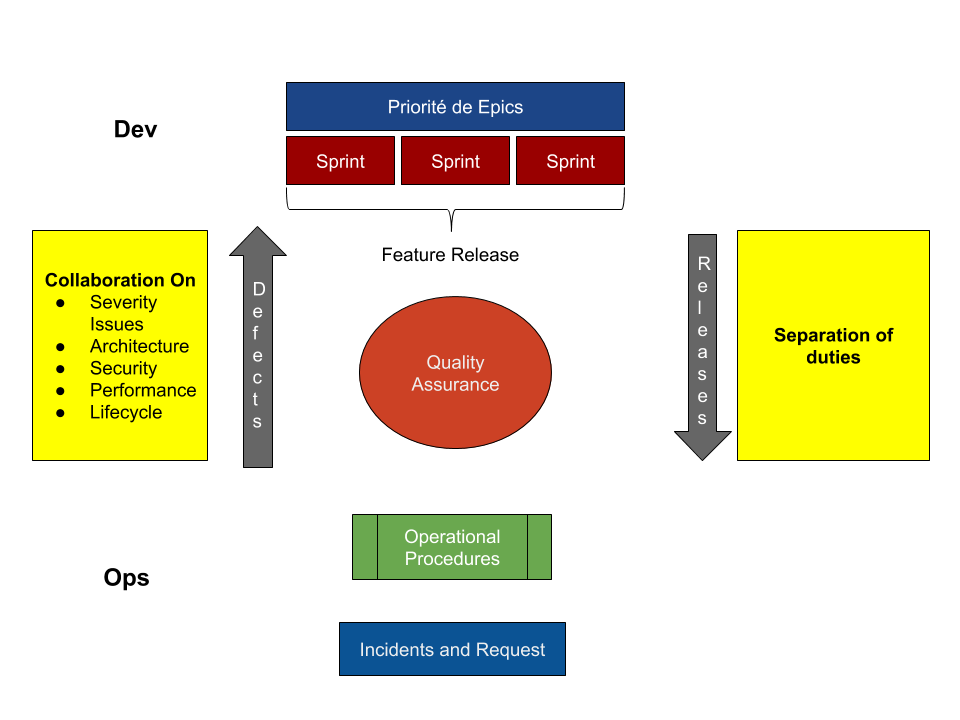
\includegraphics[scale=0.45]{devops_operational_model.png}
\caption{Modèle Opérationnel \cite{IsaacSacolick2016DrivingCulture}}
\label{devops_operational_model}
\end{figure}


\subsubsection{Acteurs}
Dans la Figure \ref{devops_operational_model} nous voyons trois acteurs principaux dans cette conversation:

\subparagraph{QA}
C'est une équipe composée par des personnes avec distinctes disciplines qui doivent travailler avec \textit{Dev} pour développer et automatiser les test.
\subparagraph{Dev} L'équipe doit livrer les livrables avec des \emph{runbooks} et d'assurer que les amélioration opérationnelles sont priorité.
\begin{itemize}
  \item Le 30\% d'un sprint doit cibler des défets téchniques.
  \item Cibler le \emph{développement complet}, c'est-à-dire, le développement prêt pour les tests de \textit{QA}.
  \item Collabore activement avec \textit{Ops}.
  \item Assurer que l'application récolte des données qui aident à l'amélioration.
\end{itemize}
\subparagraph{Ops}
L'équipe doit fournir des services dans le cloud pour permettre \textit{Dev} être plus agile et lui permettre d'apprendre à résoudre la plupart des problèmes de production.


\subsection{Le Défi}
Dans la Section \ref{sec:devops}, nous avons listé les activités de transition DevOps qui sont aussi des pratiques que \emph{BCD} vise à donner aux clients de Bonita. Figure \ref{fig:dev-to-prod}

\begin{figure}[!ht]
\centering
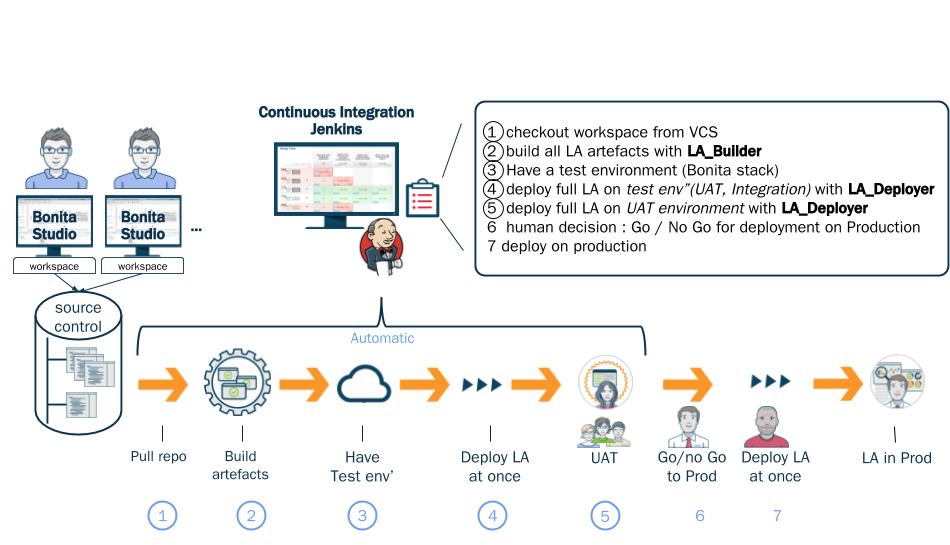
\includegraphics[width=\textwidth,keepaspectratio]{dev-to-prod.png}
\caption{Dev à Prod}
\label{fig:dev-to-prod}
\end{figure}

Les technologies utilisées actuellement sont:
\begin{itemize}
  \item Ansible
  \item Python
  \item Docker
  \item Jenkins
  \item Cloud (AWS)
\end{itemize}

Pour cette mission, j'ai dû approfondir mes connaissances sur:
\subparagraph{DevOps} De nouvelles approches qui incluent l'Intégration Continue (CI), le Déploiement Continu (CD).
\subparagraph{Agile} La communication dans un environnement agile avec les rituels.
\subparagraph{Python} Comme un langage complet avec le paradigme OO avec TDD comme méthodologie.
\subparagraph{Docker} Les bonnes pratiques pour créer une image, et comment nous pouvons les utiliser pour déployer plus rapidement des applications.
\subparagraph{Jenkins} L’architecture et le langage DSL pour  créer des "jobs" et "pipelines" pour automatiser les tests, la compilation, l’empaquetage d'un produit final.
\subparagraph{AWS} Tous les nombreux services et la façon de nous en servir.


\subsection{Chronologie}
Toutes les livraisons de tous les produits suivent le "Software Development life cycle" (SDLC). Tous les six mois une version est livrée et une fois par mois une version de maintenance est livrée.

\begin{figure}[!ht]
\centering
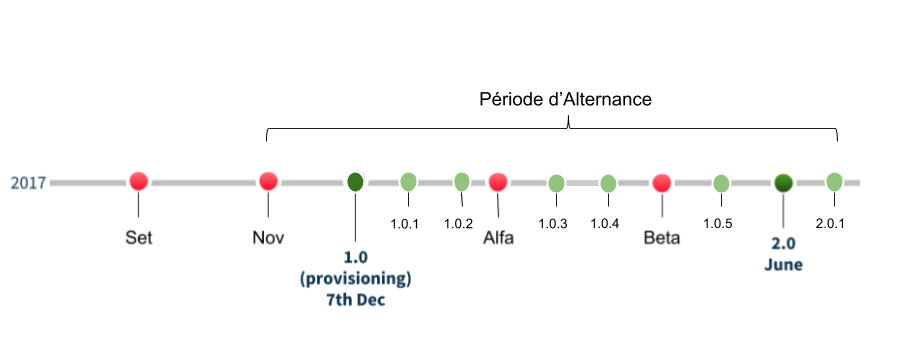
\includegraphics[scale=0.45]{bcd_my_chrono.png}
\caption{Cycle de vie}
\label{bcd_my_chrono}
\end{figure}

La Figure \ref{bcd_my_chrono} présente la période où j'ai apporté ma contribution. Les deux premièrs mois (septembre et octobre), j'ai suivi des formations sur Bonita et j'ai eu le temps d’aborder plus en détail toutes les parties du produit \emph{BCD} et les technologies utilisées.


\subsection{Travail réalisé}\label{sec:work_done}
Nous avons vu dans dans la Figure \ref{frame_safe} le chemin suivi pour la création et la définition des \textit{Epics}, \textit{Millestones} et le \textit{Backlog}. Dans la Figure \ref{fig:backlog} nous pouvons regarder un exemple du contenu Backlog.

Pendant le déroulement de mon alternance, j'ai travaillé sur plusieurs items du \textit{Backlog}. Appendice  \ref{appen:my_backlog}. Chaque item était bien découpé de sorte que la tâche puisse se terminer dans le délai d'un \textit{Sprint}.

\begin{figure}[!ht]
\centering
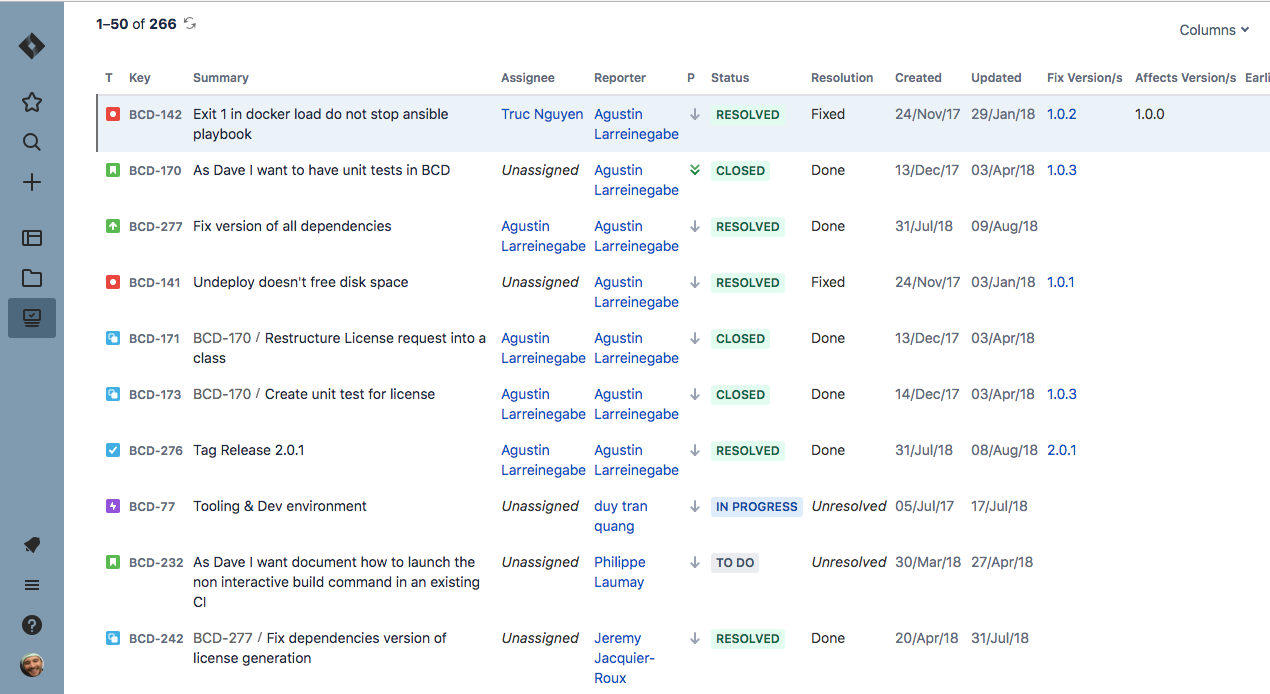
\includegraphics[width=\textwidth,keepaspectratio]{backlog.png}
\caption{Exemple Backlog}
\label{fig:backlog}
\end{figure}

Pour cela, je devais effectuer des actions différentes comme:

\subparagraph{Python} Développer et maintenir les scripts du Command Line Interface (CLI) de BCD.
\begin{itemize}
  \item J'ai participé à la réorganisation du code pour le rendre plus modulaire.
  \item J'ai participé à l'élaboration des tests unitaires pour le module BCD.
  \item J'ai participé au développement du module de \enquote{Licensing}.
\end{itemize}

\subparagraph{AWS} Une partie de BCD gère des instances dans le cloud, aussi l'entreprise a passé d'autres services sur le cloud.
\begin{itemize}
  \item J'ai aidé à implémenter le service \enquote{Organization} de AWS.
  \item J'ai dû m'impliquer plus dans les services EC2, Lambda, S3, RDS.
\end{itemize}

\subparagraph{Ansible} Développer et maintenir des \enquote{Playbook} Ansible.
\begin{itemize}
  \item J'ai participé à l'adaptation des scripts pour supporter le nouveau dépôt privé d'images docker.
\end{itemize}

\subparagraph{Jenkins} Exécution de jobs pour l'empaquetage de livrables.

\subparagraph{Git} Gestion du dépôt privé.
\begin{itemize}
  \item Revue de \enquote{Pull Request}
  \item \enquote{Merge} dans la branche correspondante.
  \item \enquote{Tag} et livre des nouvelles versions.
\end{itemize}

\subparagraph{Docker} Maintenir des images et l'investigation des nouvelles caractéristiques.

\subparagraph{Activités collatérales} Pour mieux organiser le travail en équipe, nous suivons des rituels Agile
\begin{itemize}
  \item Le \enquote{Daily Meeting} pour faire le point sur les tâches effectuées et communiquer sur les difficultés rencontrées.
  \item La \enquote{Rétrospective}, pour s’améliore.
  \item La \enquote{Réunion hebdomadaire},  elle réunit toutes les parties prenantes du projet pour faire le point sur son avancement. Ainsi, tous les participants peuvent se rendre compte si l’état du projet correspond à leurs besoins, attentes ou objectifs.
  \item \enquote{Les estimations}, où nous faisons des hypothèses à échelle relative, pour estimer une charge de travail par exemple. Cette réunion est importante pour déterminer correctement la complexité et la valeur apportée de la tâche à réaliser pour effectuer une estimation de bonne qualité.
  \item \enquote{La sélection}, où nous déterminons efficacement la charge de travail à accomplir définie dans le backlog lors de l'itération.
\end{itemize}

\subsubsection{Gestion de risques}
Il y a toujours plusieurs risques associés au développement du logiciel. Dans cette sous-partie, nous allons voir quelques risques que j'ai vu s'atténuer en comparaison à d'autres expériences de travail (pas Agile). \cite{basile_plessis_2014}
\begin{center}
\begin{tabular}{p{3cm}|p{3cm}|l|l|p{5cm}}
Description & Conséquence & Probabilité & Impact & Action \\ \hline
Prévision de travail pas juste & Rien livrer du tout & Faible & Fort & Le \enquote{Daily Metting} permet de s'assurer que sa prévision de \enquote{Sprint} est toujours d'actualité \\
Baisse de qualité du code & Bogue introduit & Modéré & Fort & Mise en place de CI, revues de code avant de l'ajouter dans la branche principale, test unitaire \\
Perte d'engagement de l'équipe & Équipe démotivée, et baisse de performance & Faible & Fort & La \enquote{Retrospective} suite de chaque \enquote{Sprint} aide l'équipe à s'améliorer. \\
Incompréhension des fonctionnalités & Ne pas livrer les bonnes fonctionnalités ou celles qui n'apportent pas de valeur & Faible & Modéré & Le \enquote{Spring Planning} permet à l'équipe de choisir les \enquote{stories} et s'engager. \\


\end{tabular}
\end{center}


\subsection{Travail qui reste}
Nous avons dit que BCD est né d'un besoin interne et des retours de clients, c'est ainsi que les fonctionnalités demandées augmentent et que le produit est toujours en évolution pour fournir au client une meilleure expérience quand il développe avec Bonita. Appendice \ref{appen:backlog}


\subsection{Les Compétences acquises}
Nous avons dans la Section \ref{sec:work_done} les outils et technologies que j'ai eu l'opportunité de toucher du doigt.
Pourtant, je ne peux pas dire que j'aie approfondi seulement le côté technologique et technique, parallèlement, j'ai amélioré mes aptitudes communicatives.


\subsection{Bilan}
Cette période d'alternance chez Bonitasoft m'a apporté une nouvelle expérience professionnelle. Grâce à cette année, j'ai acquis de nouvelles connaissances autant dans le domaine fonctionnel que dans les techniques.

Parmi les difficultés rencontrées, le travail sur un code qui existait déjà avec un langage que je ne connaissais pas en profondeur. L'acquisition des connaissances sur les nouvelles techniques et  technologies ont été aussi une entrave mais à la fois, un défi intéressant et enrichissant qui m'a beaucoup plu.

Cette expérience m'a permis d'affuter mes compétences grâce à l'intégration dans une équipe humaine et dynamique qui a été un véritable catalyseur et une source inépuisable de connaissances et d'expériences.


\subsection{Réflexion finale}
Cette formation en alternance m'a permis d'obtenir beaucoup de compétences et de savoir-faire, que ce soit sur le plan informatique avec la multitude de nouvelles technologies abordées, ceci s'ajoutant aux connaissances déjà acquises que j'ai pu approfondir. Mais également sur le plan personnel, toute la confiance qui, dès mon arrivée, m'a été donnée par l'équipe ; ma liberté d'expression et de prise de décisions ainsi que le partage d'expériences avec les collègues ont été très enrichissants et formateurs.



\section{Conclusion}
Cette expérience a été passionnante et enrichissante d'une part, grâce à l'équipe humaine qui donne tout son potentiel tous les jours, et pas seulement pour être efficace dans le travail, mais aussi pour construire une ambiance de croissance, d'amélioration et de support.
D'autre part, parce que grâce à la mission, j'ai pu approfondir mes connaissances sur la culture DevOps, ses enjeux, sa difficulté et ses bénéficies.

\section{Remerciements}
Pour clore mon rapport, je souhaiterais adresser mes remerciements en premier à ma famille et à ma copine qui m'ont toujours apporté leur soutien, ainsi qu’au Programme BECAL pour son financement et la confiance qui m'a été donnée pendant deux ans.

Je tiens aussi à remercier toute l'équipe avec laquelle j'ai eu le plaisir de travailler :
\begin{itemize}
  \item[] mon maître de stage Duy Trang Quang pour m’avoir toujours fait confiance,
  \item[] Jérémy Jacquier-Roux pour son amitié et ses conseils,
  \item[] Truc Nguyen pour sa rigueur.
\end{itemize}
Ils sont toujours été à l'écoute lorsque j'avais une question ou une proposition.

Je remercie également mon tuteur Olivier Gruber pour le temps qu’il m’a consacré cette année et pour tous les conseils qu’il m’a donnés.

Je tiens finalement à remercier tous mes collègues de Bonitasoft pour leur convivialité, pour l’ouverture et l'esprit d'amélioration continue qu’ils ont partagés avec moi cette année.



\newpage
\addcontentsline{toc}{section}{Références}

\newpage
\begin{appendices}
\section{Backlog}\label{appen:backlog}
Jira Backlog

\newpage
\section{Contribution Git}\label{appen:git_contribution}
GITHUB
\end{appendices}


\newpage
\bibliographystyle{plain}
\bibliography{reportbiblio}
\end{document}
